\documentclass{article}
\usepackage[utf8]{inputenc}
\usepackage{amsfonts, booktabs, siunitx, listings, graphicx}
\graphicspath{{./images/}}
\usepackage{booktabs}
\usepackage{siunitx}
\usepackage{graphicx}
\usepackage{listings}
\title{\textbf{Mathematical Problem Solving with Transformer Models}\\ Deep Learning Lab}
\author{Felix Boelter }
\date{\today}
\begin{document}

\maketitle
\clearpage
\section{Mathematical Problem Solving with Transformer Models}
\subsection{Problem Setups and Preliminaries}
\textbf{1)} \\The numbers - place value preprocessed dataset was downloaded, train.x corresponds to the questions,
train.y corresponds to the answers and train.xy corresponds to the questions and answers.\\\\
\textbf{2)}\\
\begin{table}[ht]
\caption{Dataset}
\begin{center}
\begin{tabular}{ccc} \toprule
   \textbf{Numbers - place value}& \textbf{Training Dataset} & \textbf{Validation Dataset} \\ \midrule
    
    Sentences  & 1999998 & 10000\\
    Characters  & 78429947 & 413219 \\
    Average Question Length  & 40 & 42  \\
    Average Answer Length & 1 & 1  \\\bottomrule
\end{tabular}
\end{center}
\end{table}
\\\\
\textbf{3)}\\
Including the start of sequence token, end of sequence token, padding token and the whitespace our vocabulary size for the source field was 33 and the vocabulary size for the target field was 14, in the numbers - place value dataset.

\subsection{Dataloader}
A source field and target field were created using  \textbf{Field} from torchtext. Using the \textbf{TranslationDataset}, the training and validation datasets were created. The vocabulary was then built on the training dataset, and a training iterator and a validation iterator were created using the \textbf{Iterator} from torchtext. The batch size was set at 128 for the training iterator and 64 for the validation iterator, for faster training.
\clearpage
\subsection{Model}
\begin{table}[ht]
\caption{Model Initialization Parameters}
\begin{center}
\begin{tabular}{cc} \toprule
   \textbf{Model Initialization}& \textbf{Parameters}\\ \midrule
    
    \begin{tabular}{@{}c@{}}\textbf{Embedding}\\ \textbf{(Source and Target)} \end{tabular} & \begin{tabular}{@{}c@{}}Tokens\\ Embedding Size\end{tabular}\\ \midrule
    \textbf{Positional Encoding}  & Hidden Dimension \\ \midrule
    \textbf{Transformer}  & \begin{tabular}{@{}c@{}}Hidden Dimension\\ Number of Heads\\ Number of Encoder Layers\\Number of Decoder Layers\\ Feed-forward dimension\\\end{tabular}  \\ \midrule
    \textbf{Fully-Connected Layer} & \begin{tabular}{@{}c@{}}Hidden Dimension\\ Target Tokens\end{tabular} \\\bottomrule

\end{tabular}
\end{center}
\end{table}
\begin{table}[ht]
\caption{Model Forward Parameters}
\begin{center}
\begin{tabular}{cc} \toprule
   \textbf{Model Forward}& \textbf{Parameters}\\ \midrule
    \begin{tabular}{@{}c@{}}\textbf{Embedding}\\ \textbf{(Source and Target)} \end{tabular} & \begin{tabular}{@{}c@{}}Vocabulary Tokens\end{tabular}\\ \midrule
    \textbf{Positional Encoding}  & Embedding \\ \midrule
    \textbf{Transformer}  & \begin{tabular}{@{}c@{}}Positional Encoded Source\\ Positional Encoded Target\\ Target Mask\\ Source key padding mask\\ Target key padding mask\\Memory key padding mask\end{tabular}  \\ \midrule
    \textbf{Fully-Connected Layer} & \begin{tabular}{@{}c@{}} Transformer Output\end{tabular} \\\bottomrule
\end{tabular}
\end{center}
\end{table}
\clearpage
\subsubsection*{Masks}
To create the target masks, I used the generate square subsequent mask from the Transformer. There was no need to create a source mask as the decoder was allowed to see the input. \\
For the key padding masks, I created a function which checked if each value of the batch is a pad token and if it is it would output a True, so that we mask it, otherwise it will output a False which will not mask it.
\subsection{Greedy Search}
The greedy search algorithm was implemented as:
\begin{enumerate}
    \item Create a target tensor with init tokens.
    \item Embed and Positional Encode the source.
    \item Create the source key padding mask.
    \item Run the positional encoded source and the source key padding mask through the encoder from nn.Transformer.
    \item Generate masks and positional encoding for the target at each decoding step.
    \item Run the memory encoded sentence from (4), positional encoded target, the target key padding mask, the target mask and the memory key padding mask through the decoder.
    \item Run the output of the decoder through a fully-connected layer.
    \item Get the argmax of the most probable prediction.
    \item Concatenate the target with the argmax from (8).
    \item Go back to (5).
\end{enumerate}
\subsubsection{Stopping criteria}
For the stopping criterion I checked if a eos token was predicted, if not I checked if the sequence length exceeded the target sequence length given from the model. If there is no target sequence length given, then the greedy search would continue till it found an EOS token, this is useful if the model is given a sentence from the validation set.
\subsubsection{Batch mode evaluation}
For fast evaluation, I used the batch mode variation for the greedy search. The things that changed were:\\
1) Target tensor was created with a batch size amount of init tokens. E.g. with a batch size of 64 there would be 64 init tokens in the the target tensor.\\
8) For the argmax I got all the predictions for the whole batch and I concatenated them to all the init tokens in the target batch.
\\
For the stopping criteria in batch mode I checked if all of the predictions had a eos token, if not I still checked if the sequence length exceeded the target sequence length.
\subsubsection{Implementation of nn.Transformer when considering its usage in a search algorithm}
nn.Transformer is based on the original paper "Attention is all you need, 2017", which implemented a Encoder/Decoder network. In a search algorithm we don't need to encode our input sentence at every time-step which is what nn.Transformer does when it is not forwarded separately.
\subsection{Accuracy Computation}
For the accuracy, I added up the total size of every batch which was given to the model. I then took the argmax of the output of the model, which I then checked against the validation labels, it returned True if the prediction matched the validation label in that position or if the validation label matched a pad token in that position. If all of the positions in that batch were True, I returned a 1 for that prediction in the batch if not I returned a 0. I then took the sum of all these numbers and added it to my correct counter.\\
The validation accuracy was then computed by taking the sum of correct values and dividing it by the total number of questions it went through.
\subsection{Training}
For the loss function I decided to use a CrossEntropyLoss.\\
Every 500 steps, I ran the validation and then printed out the accuracy on both my validation and training data subsets. I also printed out the training and validation losses, aswell as testing the model on three different sentences while getting the generated answer for each of them.\\
For the training I used gradient accumuluation, which, for a training batch size of 128 I would call optimizer.step() followed by optimizer.zero\_grad every 5 batches, which results in an effective batch size of 640.
\clearpage
\subsection{Experiments}
\begin{table}[ht]
\caption{Training hyper-parameters for \textbf{numbers - place value}}
\begin{center}
\begin{tabular}{cc} \toprule
   \textbf{Hyper Parameters} & \textbf{Parameter Values}\\ \midrule
    
    \textbf{Effective batch size} & 640\\ \midrule
    \textbf{Learning rate}  & $10^{-4}$ \\ \midrule
    \textbf{Gradient clipping rate}  & 0.1  \\ \midrule
    
    \textbf{Hidden dimension}  & 256  \\
    \textbf{Feedforward dimension}  & 1024  \\
    \textbf{Heads}  & 8  \\
    \textbf{Decoder layers}  & 2 \\
    \textbf{Encoder layers} & 3 \\\bottomrule
\end{tabular}
\end{center}
\end{table}
\begin{figure}[h]
\begin{center}$
\begin{array}{cc}
    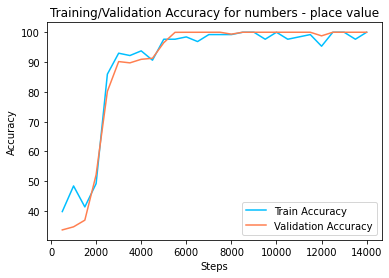
\includegraphics[scale=0.5]{Numbersplace_acc.png} &
    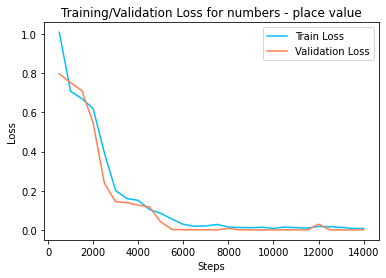
\includegraphics[scale=0.5]{Numbersplace_loss.png} 
\end{array}$
\end{center}
\caption{Training and Validation Loss/Accuracy for numbers - place value}
\end{figure}
\begin{lstlisting}[breaklines]
Example Question: What is the tens digit of 93283843? | Expected Answer: 4 | Generated Answer: 4<eos>

Example Question: What is the units digit of 93215897? | Expected Answer: 7 | Generated Answer: 7<eos>

Example Question: What is the thousands digit of 58179700? | Expected Answer: 9 | Generated Answer: 9<eos>
\end{lstlisting}
\clearpage
The training/validation accuracy both were at 100\% accuracy after 14000 steps, however the validation accuracy converged much faster and got to 100\% accuracy after only 6000 steps. The trained model also generated the expected answer to the questions perfectly every $n$ steps.
\subsubsection{Hyper-parameter Tuning}
\begin{table}[ht]
\caption{Hyperparameter Tuning for the Models}
\begin{center}
\begin{tabular}{cccccc} \toprule
   \textbf{Model} & \textbf{Hidden dim}& \textbf{Feedforward dim}
   & \textbf{Heads}& \textbf{Decoder layers}& \textbf{Encoder layers}\\ \midrule
    
    \textbf{Model 1}  & 256  & 1024 & 8 & 2 & 3\\
    \textbf{Model 2}   & 128  & 256 & 8 & 1 & 1\\
    \textbf{Model 3}   & 256  & 256 & 8 & 2 & 2 \\
    \textbf{Model 4}   & 256  & 512 & 8 & 2 & 2 \\
    \textbf{Model 5}  & 256  & 1024 & 8 & 2 & 2 \\\bottomrule
\end{tabular}
\end{center}
\end{table}
\begin{figure}[h]
\begin{center}$
\begin{array}{cc}
    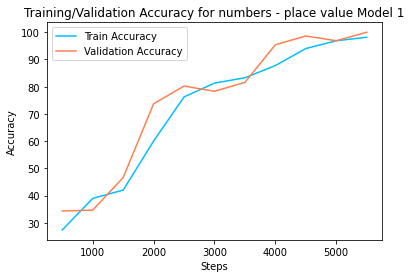
\includegraphics[scale=0.5]{Model1_default_acc.png} &
    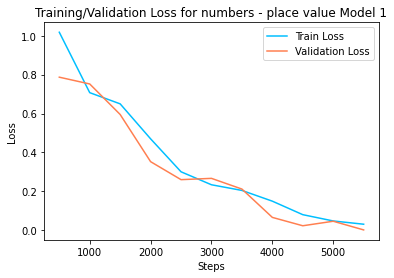
\includegraphics[scale=0.5]{Model1_default_loss.png}\\
    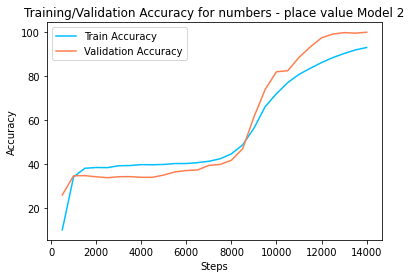
\includegraphics[scale=0.5]{model2_acc_128_256_1_1.png.png} &
    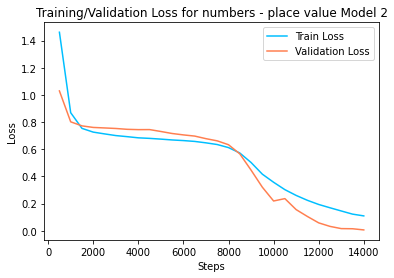
\includegraphics[scale=0.5]{model2_loss_128_256_1_1.png} \\
    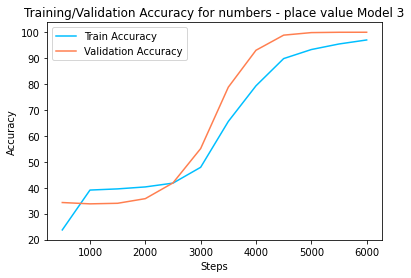
\includegraphics[scale=0.5]{model3_acc_256_256_2_2.png} &
    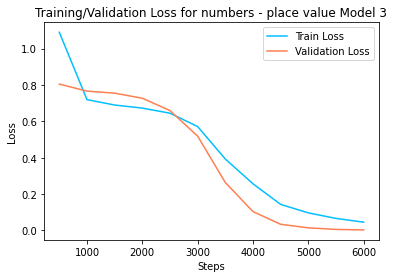
\includegraphics[scale=0.5]{model3_loss_256_256_2_2.png} \\
    
\end{array}$

\end{center}

\caption{Hyperparameter Tuning for Models 1 - 3}

\end{figure}

\begin{figure}[h]

\begin{center}
$
\begin{array}{cc}
    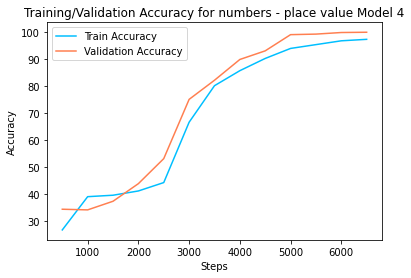
\includegraphics[scale=0.5]{model4_acc_256_512_2_2.png.png} &
    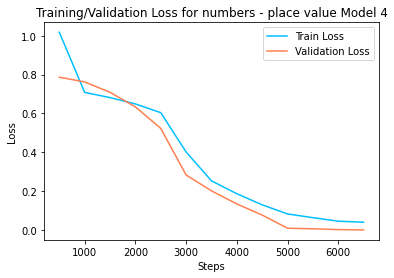
\includegraphics[scale=0.5]{model4_loss_256_512_2_2.png} \\
    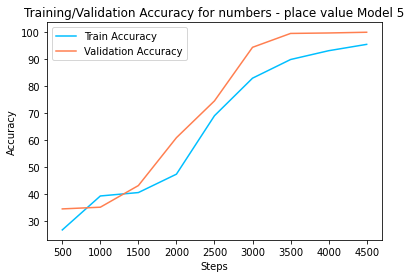
\includegraphics[scale=0.5]{model5_acc_256_1024_2_2.png} &
    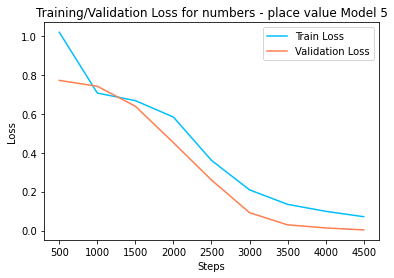
\includegraphics[scale=0.5]{model5_loss_256_1024_2_2.png}
    
\end{array}$

\end{center}

\caption{Hyperparameter Tuning for Models 4 - 5}

\end{figure}

\clearpage
Model 1 is the default model with the model size that was given, which got to 100\% validation accuracy in 6000 steps. When reducing the model to the Hyper-parameters in Model 2, it still got to 100\% validation accuracy, but at a much slower rate. The fastest rate, in which we could reduce the model size and get to 100\% validation accuracy in less steps than the default Model, was Model 5, where we got to 100\% validation accuracy in just 4500 steps.

\subsubsection{\textbf{compare - sort}}
For the compare - sort dataset, I used the same hyperparameters from Model 1 in the previous \textbf{numbers - place value} dataset.

\begin{figure}[h]
\begin{center}
$
\begin{array}{cc}

    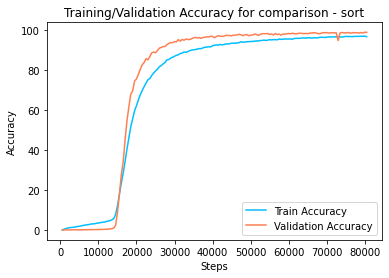
\includegraphics[scale=0.5]{comparison_acc.png} &
    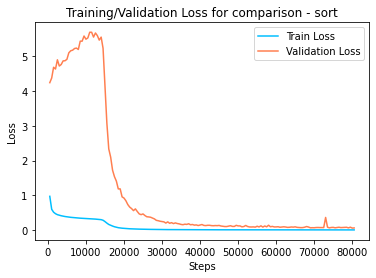
\includegraphics[scale=0.5]{comparison_loss.png} \\
    
\end{array}$

\end{center}

\caption{Training and Validation Loss/Accuracy for comparison - sort}

\end{figure}
\begin{lstlisting}[breaklines]
Example Question: Put 0.4, 5, 30, 50, -2, 16 in descending order. | Expected Answer: 50, 30, 16, 5, 0.4, -2 | Generated Answer: 50, 30, 16, 5, 0.4, -2<eos>

Example Question: Sort -25/127, -2/13, 0.2. | Expected Answer: -25/127, -2/13, 0.2 | Generated Answer: -25/127, -2/13, 0.2<eos>

Example Question: Sort 3, -0.2, 927897, 3/7 in ascending order. | Expected Answer: -0.2, 3/7, 3, 927897 | Generated Answer: -0.2, 3/7, 3, 927897<eos>
\end{lstlisting}
As can be seen from the loss graph, the task is substantially harder than \textbf{numbers - place value}, as the validation loss is going up in the first 20000 steps and then goes down sharply. Additionally, it is also harder as there are different tokens in the target sequence like , or / or decimals. Additionally, as there are different lengths in the target sequences for this dataset, there needed to be an account for padding tokens, when computing the accuracy and loss.

\subsubsection{\textbf{algebra - linear 1d module}}
The hyper-parameters I used for the algebra - linear 1d module, were different from the initial model 1 hyper-parameters.
\begin{table}[ht]
\caption{Hyper-parameters for algebra - linear 1d}
\begin{center}
\begin{tabular}{cccccc} \toprule
   \textbf{Model} & \textbf{Hidden dim}& \textbf{Feedforward dim}
   & \textbf{Heads}& \textbf{Decoder layers}& \textbf{Encoder layers}\\ \midrule
    Model 6 & 512  & 2048 & 8 & 6 & 6\\\bottomrule
\end{tabular}
\end{center}
\end{table}
\begin{figure}[h]
\begin{center}
$
\begin{array}{cc}

    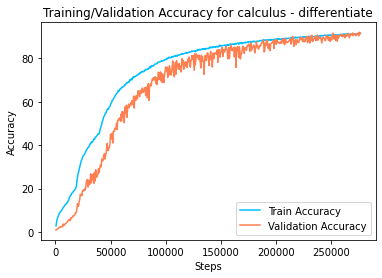
\includegraphics[scale=0.5]{calc_acc.png} &
    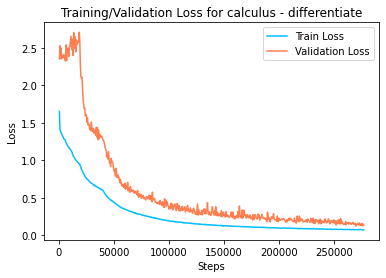
\includegraphics[scale=0.5]{calc_loss.png} \\
    
\end{array}$

\end{center}

\caption{Training and Validation Loss/Accuracy for algebra - linear 1d}

\end{figure}

\begin{lstlisting}[breaklines]
Example Question: Solve -282*d + 929 - 178 = -1223 for d. | Expected Answer: 7 | Generated Answer: 7<eos>

Example Question: Solve 0 = -i - 91*i - 1598*i - 64220 for i. | Expected Answer: -38 | Generated Answer: -38<eos>

Example Question: Solve -25*m - 2084 = -2559 for m. | Expected Answer: 19 | Generated Answer: 19<eos>
\end{lstlisting}
The module was very difficult to train as it took a lot of time. I implemented a save state and load state function to save my model data from crashing.\\
In the accuracy graph, we can see that the accuracy hits around 90\%, while the loss get's closer and closer to zero. The hyperparameter choice in my opinion went quite well, as the model keeps on learning and never seems like it will be underfitting, as it would if the model size was kept very small.
\end{document}

